\section{Constrained Generation}
\label{section:constrainedgen}

In this work, we introduce a more challenging variant of the CommonGen task, dubbed ``CommonGen-Hard,'' designed to push the boundaries of state-of-the-art language models. CommonGen-Hard requires models to generate coherent and grammatically correct sentences incorporating 20-30 concepts, as opposed to the original task which presents a set of 3-5 related concepts. This significant increase in the number of concepts tests the model's ability to perform advanced commonsense reasoning, contextual understanding, and creative problem-solving, as it must generate meaningful sentences that encompass a broader range of ideas. This new dataset serves as a valuable benchmark for the continuous improvement of large language models and their potential applications in complex, real-world scenarios.

The increased complexity of the CommonGen-Hard task makes it an ideal testbed for evaluating the effectiveness of our proposed framework, \ours, which focuses on iterative creation with introspective feedback. Given that initial outputs from language models may not always meet the desired level of quality, coherence, or sensibility, applying \ours enables the models to provide multi-dimensional feedback on their own generated output and subsequently refine it based on the introspective feedback provided. Through iterative creation and self-reflection, the \ours framework empowers language models to progressively enhance the quality of their output, closely mimicking the human creative process and demonstrating its ability to improve generated text on complex and demanding natural language generation tasks like CommonGen-Hard (\autoref{fig:commongen_results}).

\begin{figure}
\centering
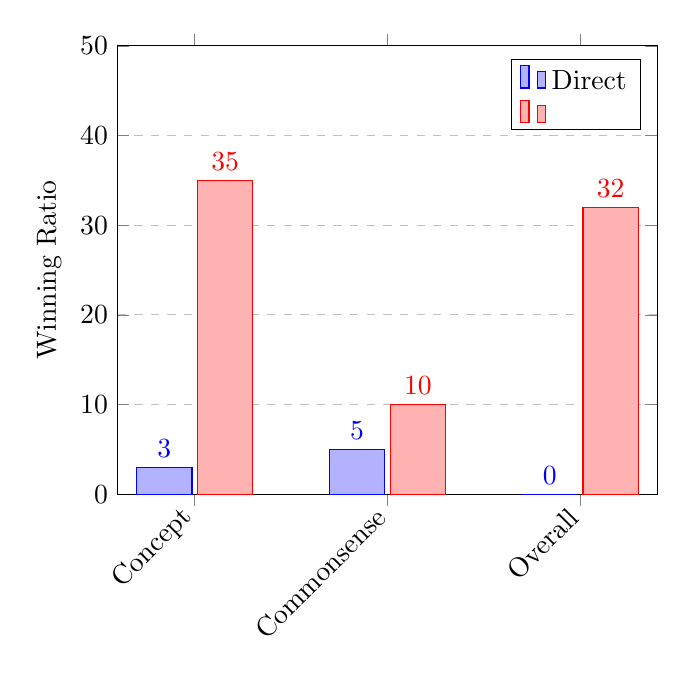
\begin{tikzpicture}
\begin{axis}[
    ybar,
    enlarge x limits=0.2,
    ylabel={Winning Ratio},
    symbolic x coords={Concept, Commonsense, Overall},
    xtick=data,
    x tick label style={rotate=45, anchor=east},
    legend pos=north east,
    bar width=20pt,
    nodes near coords,
    ymin=0, ymax=50,
    ytick={0, 10, 20, 30, 40, 50},
    ymajorgrids=true,
    grid style=dashed,
]
\addplot coordinates {(Concept, 3) (Commonsense, 5) (Overall, 0.00)};
\addplot coordinates {(Concept,  35) (Commonsense,  10) (Overall,  32)};
\legend{Direct, \ours}
\end{axis}
\end{tikzpicture}
\caption{A comparison of \ours and direct generation with \gptt on CommonGen-Hard.}
\label{fig:commongen_results}
\end{figure}